% ACL 2027 submission
% Does Language Matter? Evaluating LLM-Agent Performance Across Languages
\documentclass[11pt]{article}
\usepackage[review]{acl}   % use [review] for anonymous submission; drop it for camera-ready
\usepackage{times}
\usepackage{latexsym}
\usepackage[T1]{fontenc}
\usepackage[utf8]{inputenc}
\usepackage{microtype}
\usepackage{graphicx}
\usepackage{booktabs}
\usepackage{array}
\usepackage{amsmath}
\usepackage{multirow}
\usepackage{enumitem}
\usepackage{xcolor}
\usepackage{url}

\newcommand{\dn}[1]{\textcolor{red!70!black}{#1}}
\newcommand{\up}[1]{\textcolor{green!45!black}{#1}}
\newcolumntype{L}[1]{>{\raggedright\arraybackslash}p{#1}}

\title{Does Language Matter? \\ Evaluating LLM-Agent Performance Across Languages}

\author{Anonymous ACL submission}

\begin{document}
\maketitle

\begin{abstract}
LLM agents are increasingly deployed to carry out multi-step, tool-using work, yet they are
evaluated almost exclusively in English. We ask a simple question with a non-obvious answer:
when the \emph{same} task is expressed in a different language, does the agent behave
differently, and if so, \emph{where} in its pipeline?
We build paired English/Bangla versions of four agent benchmarks---\textsc{OfficeBench},
$\tau^2$-bench, \textsc{WorkBench} and \textsc{TheAgentCompany}---holding the environment, the
tool schema and the checkers fixed while varying only the language of the instructions (and,
where present, of the simulated user), and we run two open-weight models (31B and 20B
parameters). On \textsc{OfficeBench} (300 subtasks per condition) the effect of language is
\textbf{model-dependent in direction}: the 31B model loses $8.0$ points in Bangla ($p{=}0.003$,
exact McNemar) while the 20B model \emph{gains} $6.7$ points ($p{=}0.022$), so the gap between
the two models shrinks from $21.6$ points in English to $7.0$ in Bangla.
A failure-mode analysis explains the divergence. The 31B model's failures are
\emph{content-bound}; the 20B model's are \emph{action-format-bound}---$97\%$ of its English
failures involve a malformed action---and the language shift reduces the prose leakage that
causes them.
Across all four benchmarks, only 24 of 163 hand-analysed Bangla-only failures are genuine Bangla
agent failures; the rest come from English-only checkers, the Bangla user simulator, translation,
the harness, or weaknesses that also occur in English. Removing these benchmark-side confounds
on both sides puts every significant gap inside its confidence interval around zero. On
\textsc{OfficeBench}, $27\%$ of the 31B model's Bangla failures are answers written in Bangla
script and rejected by English keyword checkers; crediting them would raise its Bangla score
above its English score. We argue that multilingual agent evaluation requires language-aware
verification, and we release code, traces and failure codes.
\end{abstract}

\section{Introduction}

\begin{figure*}[t]
\centering
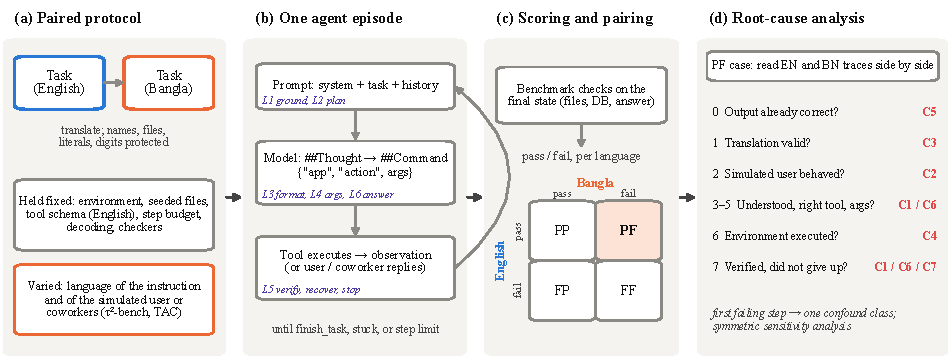
\includegraphics[width=\textwidth]{figures/fig_overview.pdf}
\caption{Study overview. (a) Each task runs once in English and once in Bangla; only the
language of the instruction (and of the simulated user or coworkers, where a benchmark has
them) changes. (b) The agent loop; L1--L6 mark the layers at which a run can first fail.
(c) The benchmark's checks score each run, and the two runs of a task form one paired outcome.
(d) Every English-pass/Bangla-fail (PF) case is traced to its first failing step and given one
confound class C1--C7 (Section~\ref{sec:four}).}
\label{fig:overview}
\end{figure*}

Language-model agents now plan over many steps, call tools, and edit real artefacts---
spreadsheets, calendars, documents, email \citep{yao2023react,liu2023agentbench,zhou2024webarena}.
The benchmarks that measure them, however, are written almost entirely in English
\citep{jimenez2024swebench,xie2024osworld,mialon2024gaia}. This is a consequential gap. Most
of the world does not work in English, and an agent that edits a payroll spreadsheet is
supposed to be usable by the person who owns the spreadsheet, in that person's language.

The usual assumption is that moving a task into a lower-resource language degrades performance,
because multilingual capability lags English in knowledge and reasoning benchmarks
\citep{ahuja2023mega,shi2023mgsm,bandarkar2024belebele,huang2023notall}. For \emph{agents} this
assumption has not been tested carefully, and it hides a more interesting question. An agentic
episode is not one forward pass. It is a loop of reading state, reasoning, emitting a
structured action, and consuming the result. Language could in principle perturb any of these
stages, and a benchmark score collapses all of them into a single bit of success.

We therefore ask three questions.
\textbf{RQ1:} Does expressing an equivalent task in a different language change end-to-end
agent success, and in which direction?
\textbf{RQ2:} Where does the change act---on task understanding and content, or on the
mechanics of tool interaction?
\textbf{RQ3:} How much of an apparent cross-lingual gap is a property of the \emph{agent}, and
how much is a property of the \emph{evaluation harness}?

To answer these we construct a strictly paired bilingual protocol
(Figure~\ref{fig:overview}) over \textsc{OfficeBench}
\citep{wang2024officebench}, a benchmark of 300 office subtasks requiring one, two or three
applications. We translate only the system prompt and the task instruction into Bangla---a
language with roughly 240M speakers that is nevertheless under-represented in LLM training
data \citep{joshi2020state}---while holding the Docker environment, the file state, the tool
schema and the automatic checkers byte-identical across conditions. We evaluate two
open-weight models of comparable but distinct scale and lineage, and we code every failure.
We then apply the same paired protocol and failure analysis to three further benchmarks with
different interaction designs: customer-service dialogues with a simulated user
($\tau^2$-bench), single-turn function calling against a workplace database
(\textsc{WorkBench}), and long-horizon company tasks with simulated coworkers
(\textsc{TheAgentCompany}).

Our findings overturn the simple ``lower-resource is worse'' expectation:

\begin{itemize}[noitemsep,topsep=2pt]
\item \textbf{Direction is model-dependent.} On \textsc{OfficeBench}, \texttt{gemma4:31b} falls
from $50.3\%$ to $42.3\%$ in Bangla ($p{=}0.003$); \texttt{gpt-oss:20b} \emph{rises} from
$28.7\%$ to $35.3\%$ ($p{=}0.022$). Aggregate ``multilingual degradation'' is not a property of
the language.
\item \textbf{Model gaps do not transfer.} The English gap between the two models ($21.6$
points, $p{=}2{\times}10^{-11}$) shrinks to $7.0$ points in Bangla ($p{=}0.020$). A leaderboard
built in English overstates the difference a Bangla user would see.
\item \textbf{Failure mode predicts direction.} The models fail for different reasons. When
failures are format-bound, a language shift can help; when they are content-bound, it hurts.
\item \textbf{Evaluators are part of the measurement.} $27\%$ of the 31B model's Bangla
failures are Bangla-script answers rejected by English keyword checks. The measured language
penalty is, in large part, a property of the checker.
\item \textbf{Most Bangla-only failures are not agent failures.} Across four benchmarks, 24 of
163 hand-analysed Bangla-only failures are genuine Bangla agent failures. The dominant confound
follows the benchmark design---the checker on \textsc{OfficeBench}, the simulated user on
$\tau^2$-bench---and removing confounds on both sides brings every significant gap within
noise (Section~\ref{sec:four}).
\item \textbf{The effect depends on the type of work.} Grouping the tasks of three further
benchmarks into nine task types, failure rates differ far more between types than between
languages, and the Bangla penalty concentrates in dialogue tasks in which a Bangla-speaking
simulated user takes part (Section~\ref{sec:taxonomy}).
\end{itemize}

\section{Related Work}

\paragraph{Agent benchmarks.} Interactive benchmarks evaluate LLMs as decision makers rather
than text producers: \textsc{AgentBench} \citep{liu2023agentbench}, \textsc{WebArena}
\citep{zhou2024webarena}, \textsc{OSWorld} \citep{xie2024osworld}, \textsc{SWE-bench}
\citep{jimenez2024swebench} and \textsc{GAIA} \citep{mialon2024gaia}. \textsc{OfficeBench}
\citep{wang2024officebench} is the setting we adopt: it requires switching between office
applications and grounding actions in a real file system, and it scores outcomes with
execution-based checks rather than string overlap. $\tau^2$-bench \citep{barres2025tau2},
\textsc{WorkBench} \citep{styles2024workbench} and \textsc{TheAgentCompany}
\citep{xu2024theagentcompany} extend this to dialogue with a simulated user, workplace
databases and long-horizon company tasks; we use them in Section~\ref{sec:taxonomy}. All of
these are English-only.

\paragraph{Multilingual evaluation.} Cross-lingual evaluation of LLMs is well developed for
static tasks---\textsc{XNLI} \citep{conneau2018xnli}, \textsc{MEGA} \citep{ahuja2023mega},
\textsc{MGSM} \citep{shi2023mgsm}, \textsc{Belebele} \citep{bandarkar2024belebele}---and
consistently reports an English advantage, with the gap widening for lower-resource languages
\citep{huang2023notall,zhang2023dont}. \citet{etxaniz2024multilingual} show that models often
perform better when a prompt is first translated into English, implying an English-centric
internal pivot. These studies evaluate single-turn outputs; we ask what happens when the output
must be a \emph{valid action in a loop}.

\paragraph{Tool use and structured output.} Agents must emit well-formed, schema-conforming
calls \citep{schick2023toolformer,qin2024toolllm,patil2024gorilla}. Format adherence is itself a
capability, and it is known to be brittle. Our analysis shows that this brittleness, rather than
comprehension, dominates one of our two models and determines the sign of its language effect.

\paragraph{Failure analysis.} Rather than reporting a single score, a growing line of work
dissects \emph{how} systems fail \citep{bang2023multitask}. We follow that approach: we code
every failed episode and treat the code distribution, not the aggregate, as the object of study.

\section{Study Design}

\subsection{Benchmark and environment}
\textsc{OfficeBench} provides 300 subtasks spanning eight applications (calendar, excel, ocr,
pdf, shell, word, email, and an in-container \texttt{llm} helper). Tasks are stratified by the
number of applications required: 93 one-app, 95 two-app and 112 three-app subtasks. Each
subtask ships a seeded file system and a set of execution-based checks (cell values, file
existence, calendar overlap, keyword containment). A subtask passes only if \emph{all} of its
checks pass. Every episode runs in a fresh Docker container reset from a pinned image.

\subsection{The paired bilingual protocol}
Our central design requirement is that language be the \emph{only} variable. Concretely, across
the two conditions we hold fixed: the container image and seeded files; the available
applications; the tool schema (action names and argument keys); the step budget; the decoding
parameters; and the checkers. We vary:

\begin{enumerate}[noitemsep,topsep=2pt]
\item \textbf{The system prompt}, authored natively in Bangla, including the role description,
the application descriptions and the response-format instruction.
\item \textbf{The task instruction}, machine-translated into Bangla and cached so that every
model sees an identical string for a given subtask.
\end{enumerate}

Crucially, the \textbf{tool schema remains in English}. Action identifiers such as
\texttt{switch\_app} and argument keys such as \texttt{file\_path} are API symbols that the
executor matches literally; translating them would change the environment rather than the
language of the task, and would make the two conditions incomparable. We therefore present the
schema in English in both conditions and attach a Bangla gloss describing what each tool does.
This isolates \emph{instruction language} from \emph{interface language}, and it mirrors
deployment reality, where an interface is typically English while the user is not.

\subsection{Agent scaffold}
We use a ReAct-style loop \citep{yao2023react}. At each step the model receives the system
prompt, the task, the history of previous (action, observation) pairs, and the actions
available in the current application. It must reply with a short reasoning segment followed by
exactly one JSON action:

\begin{quote}\small\ttfamily
\#\#Thought: \textless reasoning\textgreater \\
\#\#Command: \{"app": ..., "action": ..., ...\}
\end{quote}

The harness parses the JSON after the last \texttt{\#\#Command:} marker, so reasoning may not
corrupt the action. An episode terminates when the agent emits \texttt{finish\_task}, repeats an
identical action five times (recorded as \emph{stuck}), or reaches the 20-step budget. We log the
full trajectory---prompt, reasoning, action, observation---for every step.

\subsection{Models}
We evaluate two open-weight models served through the same API with identical decoding
($\mathrm{temperature}=0$, $\mathrm{top\_p}=1$): \texttt{gemma4:31b} ($32.7$B parameters) and
\texttt{gpt-oss:20b} ($20.9$B parameters).\footnote{Served via Ollama; sizes read from the
served model metadata.} The two are deliberately different in kind: the former is a
conventional instruction-following model, the latter exposes a separate reasoning channel, and
this architectural difference turns out to drive our central result. For the reasoning model we
fold the reasoning channel into the logged \texttt{\#\#Thought} so that both conditions are
logged identically.

\subsection{Scoring}
\label{sec:scoring}
We score every episode with the benchmark's own checks after repairing three defects in the
shipped scorer: email checks now read the episode's own file system (the shipped check reads a
path that exists only inside the container); mailbox lookup tries the exact account name before
case-insensitive matches among folders that hold mail (the shipped fallback raises an error);
and text files are read as UTF-8. No check is relaxed. The repairs raise the pass counts from
132, 103, 80 and 97 to 151, 127, 86 and 106 (gemma EN, gemma BN, gpt-oss EN, gpt-oss BN) and do
not change the direction of any result; Appendix~\ref{app:repro} gives both sets.

\subsection{Metrics and statistics}
Our primary metric is the benchmark's pass rate under the repaired scorer. Because the design is \emph{paired}---the
same 300 subtasks in both conditions---we test differences with the exact two-sided McNemar
test over discordant pairs, which is the appropriate test for paired binary outcomes
\citep{mcnemar1947}. We report discordant counts ($b$, $c$) alongside each $p$-value so that
effect size is visible.

\subsection{Failure coding}
We code every failed episode from its trajectory. Besides a general taxonomy (benchmark defect,
wrong content, out of steps, premature finish, task read differently, action format), the Bangla
condition requires codes that cannot occur in English, notably \emph{answer language}: the agent
produced a semantically reasonable answer in Bangla script which an English keyword check
rejects. In addition to coding, we extract fully objective signals for all 1{,}200 episodes:
whether any action was rejected as malformed, whether the episode ended stuck, whether it
exhausted the step budget, whether it finished and still failed, episode length, and whether the
final answer contained Bangla script.

\section{Results}

\subsection{RQ1: Language changes success, but not in one direction}

Table~\ref{tab:main} gives the main result. The two models move in \emph{opposite} directions.
\texttt{gemma4:31b} drops from $50.3\%$ to $42.3\%$, an $8.0$-point loss, with 42 subtasks
passing only in English against 18 passing only in Bangla (exact McNemar $p=0.003$).
\texttt{gpt-oss:20b} moves the other way, from $28.7\%$ to $35.3\%$, a $6.7$-point gain, with 25
English-only passes against 45 Bangla-only passes ($p=0.022$).

\begin{table}[t]
\centering\small
\begin{tabular}{llcccc}
\toprule
Model & Lang & 1-app & 2-app & 3-app & All \\
 & & (93) & (95) & (112) & (300) \\
\midrule
\multirow{2}{*}{gemma4:31b}
 & EN & 67.7 & 63.2 & 25.0 & \textbf{50.3} \\
 & BN & 51.6 & 53.7 & 25.0 & \dn{42.3} \\
\midrule
\multirow{2}{*}{gpt-oss:20b}
 & EN & 44.1 & 38.9 & 7.1 & 28.7 \\
 & BN & 53.8 & 43.2 & 13.4 & \up{35.3} \\
\bottomrule
\end{tabular}
\caption{\textsc{OfficeBench} pass rate (\%) by condition and task complexity (repaired
scorer, Section~\ref{sec:scoring}). Paired exact McNemar:
gemma EN\,vs\,BN $p=0.003$ ($b{=}42$, $c{=}18$);
gpt-oss EN\,vs\,BN $p=0.022$ ($b{=}25$, $c{=}45$).}
\label{tab:main}
\end{table}

The aggregate conclusion is therefore not ``Bangla is harder''. The language manipulation is
identical; only the model differs. Any claim of the form ``model performance degrades in
language $L$'' is under-specified unless the model is named.

\paragraph{Model gaps do not transfer across languages.}
This has a direct practical consequence. In English, \texttt{gemma4:31b}
beats \texttt{gpt-oss:20b} decisively: 82 subtasks are solved only by gemma against 17 only by
gpt-oss ($p=2.2\times10^{-11}$), a gap of $21.6$ points. In Bangla the same comparison yields 48
against 27 ($p=0.020$): the ordering holds, but the gap shrinks by two thirds, to $7.0$ points.
A practitioner choosing a model from an English leaderboard would expect a far larger advantage
than a Bangla user would see.

\subsection{RQ2: Complexity gates the language effect}

Table~\ref{tab:main} also shows that the language effect is not uniform across difficulty. For
\texttt{gemma4:31b} the Bangla penalty is largest on one-app tasks ($-16.1$ points) and
\emph{exactly zero} on three-app tasks ($25.0\%$ in both conditions).

The explanation is a floor effect: both models fail most three-app workflows (OCR, summarise,
split, send mail) in either language, and where a model has no competence to lose, language
cannot take any away. A cross-lingual evaluation run only on hard tasks therefore under-reports
the language effect.

\subsection{RQ3: Failure mode determines the sign}

Why do the two models move in opposite directions under an identical manipulation? Because they
fail for different reasons (Table~\ref{tab:modes}).

\begin{table}[t]
\centering\small
\begin{tabular}{lcccc}
\toprule
 & \multicolumn{2}{c}{gemma4:31b} & \multicolumn{2}{c}{gpt-oss:20b} \\
\cmidrule(lr){2-3}\cmidrule(lr){4-5}
Signal & EN & BN & EN & BN \\
\midrule
Failures            & 149 & 173 & 214 & 194 \\
\;\;malformed action & 49 & 23 & \textbf{207} & \textbf{177} \\
\;\;ended stuck      & 3 & 5 & 30 & 14 \\
\;\;out of steps     & 46 & 39 & 81 & 58 \\
\;\;finished, failed & 99 & 128 & 102 & 121 \\
\midrule
Mean steps/episode   & 10.9 & 10.5 & 13.3 & 12.1 \\
Bangla-script answer & 0 & \textbf{46} & 0 & 7 \\
\bottomrule
\end{tabular}
\caption{Failure composition over all 300 subtasks per condition. The three terminal states
(stuck / out of steps / finished-but-failed) are mutually exclusive and sum to the failure count
together with one unsaved episode per condition; \emph{malformed action} is a cross-cutting flag
counting failures in which at least one action was rejected, so it overlaps the others. gpt-oss
is dominated by action-format failures; gemma by episodes that finish and still fail.}
\label{tab:modes}
\end{table}

\texttt{gpt-oss:20b} is \textbf{format-bound}. $207$ of its $214$ English failures ($97\%$)
contain at least one action rejected as malformed. Its reasoning lives in a separate channel,
and in English it frequently spills prose into the action slot, producing a rejected action,
then another, until the episode is consumed. Under Bangla instructions this leakage falls:
malformed-action failures drop to $177$, stuck episodes halve ($30\rightarrow14$), budget
exhaustion falls ($81\rightarrow58$), and episodes shorten ($13.3\rightarrow12.1$ steps). The
model is not understanding the task better; it is \emph{talking less} into the action channel,
and it therefore completes more episodes. Its gain in Bangla is a format effect, not a
comprehension effect.

\texttt{gemma4:31b} is \textbf{content-bound}. It emits valid actions (only $49$ of $149$
English failures involve a malformed action) and its dominant failure is an episode that runs to
completion and is then rejected on content---$99$ in English rising to $128$ in Bangla. This is
the mode that a language change should affect, and it does.

This yields a simple predictive rule, and the central claim of this paper:

\begin{quote}\itshape
The sign of an agent's cross-lingual effect follows its dominant failure mode. Content-bound
agents lose under a language shift; format-bound agents may gain, because the shift suppresses
the verbosity that corrupts their actions.
\end{quote}

\subsection{RQ4: Much of the measured penalty belongs to the evaluator}

The last row of Table~\ref{tab:modes} isolates a failure mode that \emph{cannot} occur in
English. In $46$ of its $173$ Bangla failures ($27\%$), \texttt{gemma4:31b} terminated by
calling \texttt{finish\_task} with an answer written in Bangla script. For $41$ of those
subtasks a failing check is \texttt{evaluate\_contain}, which tests whether an English keyword
occurs in the output.

The agent was asked in Bangla, answered in Bangla, and was marked wrong because the checker
was written in English---a property of the measuring instrument, not of the agent. Under the
strict checkers \texttt{gemma4:31b} scores $42.3\%$ in Bangla. If every Bangla-script answer were credited---a
deliberate upper bound, since we do not verify each one semantically---it would score $57.7\%$,
which is \emph{above} its own English score of $50.3\%$ (for \texttt{gpt-oss:20b} the bound
moves $35.3\%$ only to $37.7\%$). Reading the traces, 15 of the 42
subtasks that gemma passes only in English are of this kind: the Bangla answer has the right
content (for example ``40'' written in Bengali digits) and fails only on script; crediting just
those 15 lowers the measured gap from $8.0$ to $3.0$ points. The true value lies between the two
bounds, and we cannot determine it with English-only checkers. The honest conclusion is
therefore stronger and more useful than the naive one: \textbf{we cannot claim from these
numbers that Bangla degrades this model's task competence, because the instrument that produced
the number is itself language-biased.}

Notably the confound is itself model-dependent: \texttt{gpt-oss:20b} answered in Bangla only $7$
times, because it remains English-anchored even under Bangla instructions. A checker bias thus
penalises precisely the model that adapts to the user's language---exactly the behaviour one
would want to reward.

\section{Four Benchmarks: Results and Root Causes}
\label{sec:four}

\paragraph{Additional benchmarks.} $\tau^2$-bench \citep{barres2025tau2} consists of
customer-service dialogues (airline, retail, telecom, banking) in which an LLM-simulated
customer talks to the agent; in the Bangla condition the simulated customer also speaks Bangla.
We use 218 paired tasks for \texttt{gemma4:31b} and 149 for \texttt{gpt-oss:20b}, after removing
pairs with an infrastructure error in either language. \textsc{WorkBench}
\citep{styles2024workbench} has single-turn workplace tasks (email, calendar, analytics,
project management, CRM and multi-domain) scored by comparing the final database with the
ground truth; we use a 90-task pilot, 15 per domain. \textsc{TheAgentCompany}
\citep{xu2024theagentcompany} has long-horizon company tasks run by an OpenHands agent
\citep{wang2025openhands} with LLM-played coworkers, scored by checkpoints; we use 23
task-runs (21 tasks) with \texttt{gemma4:31b} only, and count a run as passed only when it
earns every checkpoint. The protocol is the one of Section~3.2: the instruction (and, where
present, the simulated customer or coworkers) is in Bangla, while tool names, identifiers, file
names and URLs stay in English; there is one run per cell at temperature~0.

\paragraph{Root-cause coding.} Each English-pass/Bangla-fail case gets its first failure point
(the earliest step that, corrected alone, would most likely have passed) and one confound class
from the decision tree of Figure~\ref{fig:overview}d (classes in Table~\ref{tab:confound}).
Sensitivity analyses then remove confounded tasks, on both sides where English-only failures
were coded too.

\begin{table}[t]
\centering\footnotesize
\setlength{\tabcolsep}{2.4pt}
\begin{tabular}{lrrrrr}
\toprule
 & $n$ & EN & BN & Gap [95\% CI] & $p$ \\
\midrule
OB gemma     & 300 & 50.3 & 42.3 & $+8.0$ [3.0, 13.0]      & .003 \\
OB gpt-oss   & 300 & 28.7 & 35.3 & $-6.7$ [$-$12.0, $-$1.3] & .022 \\
$\tau^2$ gemma   & 218 & 49.5 & 38.1 & $+11.5$ [5.0, 17.4]   & .001 \\
$\tau^2$ gpt-oss & 149 & 38.9 & 39.6 & $-0.7$ [$-$10.7, 8.7] & 1.00 \\
WB gemma     & 90  & 81.1 & 82.2 & $-1.1$ [$-$10.0, 7.8]   & 1.00 \\
WB gpt-oss   & 90  & 58.9 & 53.3 & $+5.6$ [$-$5.6, 16.7]   & .424 \\
TAC gemma    & 23  & 39.1 & 26.1 & $+13.0$ [0.0, 26.1]     & .250 \\
\bottomrule
\end{tabular}
\caption{Pass rate (\%) on the four benchmarks (OB: \textsc{OfficeBench}, WB:
\textsc{WorkBench}, TAC: \textsc{TheAgentCompany}, full completion). Gap: English minus Bangla,
positive when Bangla is worse; interval from a paired bootstrap over tasks (4{,}000 resamples);
$p$: exact McNemar.}
\label{tab:four}
\end{table}

\begin{table}[t]
\centering\footnotesize
\setlength{\tabcolsep}{2.6pt}
\begin{tabular}{lrrrrrrrr}
\toprule
 & \multicolumn{2}{c}{OfficeB.} & \multicolumn{2}{c}{$\tau^2$} & \multicolumn{2}{c}{WorkB.} & TAC & \\
\cmidrule(lr){2-3}\cmidrule(lr){4-5}\cmidrule(lr){6-7}\cmidrule(lr){8-8}
Confound & g & o & g & o & g & o & g & All \\
\midrule
C1 genuine Bangla    & 6  & 7 & 6  & 2  & 2 & 1  & 0 & 24 \\
C2 simulated user    & 0  & 0 & 19 & 16 & 0 & 0  & 0 & 35 \\
C3 translation       & 6  & 0 & 1  & 0  & 1 & 0  & 1 & 9 \\
C4 tool / env.       & 5  & 2 & 0  & 0  & 0 & 0  & 1 & 8 \\
C5 checker / task    & 15 & 6 & 0  & 0  & 1 & 0  & 0 & 22 \\
C6 also in English   & 3  & 1 & 14 & 7  & 3 & 14 & 3 & 45 \\
C7 unclear           & 7  & 9 & 0  & 1  & 0 & 0  & 3 & 20 \\
\midrule
Cases                & 42 & 25 & 40 & 26 & 7 & 15 & 8 & 163 \\
\bottomrule
\end{tabular}
\caption{Confound class of every hand-analysed Bangla-only failure (g: gemma4:31b, o:
gpt-oss:20b). TAC cases include Bangla reruns that disagree and both-fail tasks with different
partial scores.}
\label{tab:confound}
\end{table}

\paragraph{The language effect depends on model and benchmark.} Table~\ref{tab:four} shows a
significant Bangla penalty for \texttt{gemma4:31b} on \textsc{OfficeBench} and $\tau^2$-bench
(a second set of 219 $\tau^2$ tasks agrees: $33.8\%\to25.1\%$, $p=0.034$), a significant Bangla
\emph{advantage} for \texttt{gpt-oss:20b} on \textsc{OfficeBench}, and no detectable gap on
\textsc{WorkBench} or on the small \textsc{TheAgentCompany} pilot.

\paragraph{Most Bangla-only failures are not Bangla agent failures.} Only 24 of the 163 cases
(15\%) are genuine Bangla agent failures (Table~\ref{tab:confound}). The dominant confound
follows the benchmark's design, that is, which component reads Bangla text: English keyword
checkers on \textsc{OfficeBench} (C5), the Bangla simulated customer on $\tau^2$-bench (C2),
which often confirms an action and ends the dialogue in the same turn, and language-independent
argument errors on \textsc{WorkBench} (C6), where the tool descriptions stay in English and no
free-text answer is checked. On \textsc{TheAgentCompany} the only stable English-only pass is
again a checker artefact: the coworkers reply in Bangla and a checkpoint looks for the English
word ``helpful''.

\begin{figure}[t]
\centering
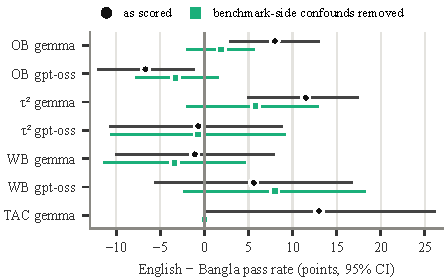
\includegraphics[width=\columnwidth]{figures/fig_forest.pdf}
\caption{English minus Bangla pass rate as scored and after removing benchmark-side confounds
(checker, translation, harness; on $\tau^2$, dialogues the simulated user ended early, in either
language; on TAC, reruns that disagree). Every significant gap moves inside an interval
containing zero.}
\label{fig:forest}
\end{figure}

\paragraph{Gaps shrink toward zero once confounds are removed.} Removing benchmark-side
confounds on both sides of the comparison (Figure~\ref{fig:forest}) moves the
\textsc{OfficeBench} gaps from $+8.0$ to $+1.9$ points (gemma) and from $-6.7$ to $-3.3$
(gpt-oss), the $\tau^2$ gemma gap from $+11.5$ to $+5.8$, and the \textsc{TheAgentCompany} gap to
zero; every interval then includes zero. This does not show that Bangla has no cost: with one
run per cell the remaining genuine cases are too few to establish or exclude a small one.

\paragraph{Two genuine mechanisms recur.} The genuine cases share two mechanisms, both seen
in both models. First, a name that appears only in Bangla script has no letter case; the agent
writes it in lower case (``bob'') for a case-sensitive mailbox or calendar lookup, receives an
empty result and accepts it (3 gemma and 6 gpt-oss \textsc{OfficeBench} cases, two of them the
same subtasks). Second, the agent renders a value back into a different English form: ``Trip''
for travelling, ``curd'' for yogurt, ``08:00 AM'' for 8:00, or a rolling seven-day window for
``last week'' on \textsc{WorkBench}. No Bangla-only $\tau^2$ failure starts with malformed tool syntax, and no
\textsc{WorkBench} tool argument contains Bangla script.

\begin{figure}[t]
\centering
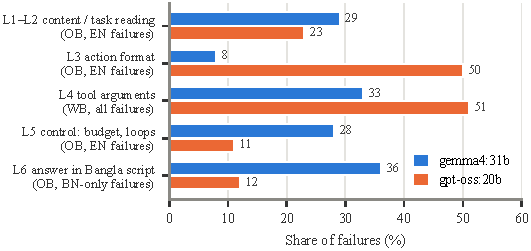
\includegraphics[width=\columnwidth]{figures/fig_layers.pdf}
\caption{Layer of the agent loop (Figure~\ref{fig:overview}b) at which failures arise, by model.
OB: \textsc{OfficeBench} (L1--L3, L5: English failures by primary root cause; L6: share of
Bangla-only failures); WB: \textsc{WorkBench}, all failed runs.}
\label{fig:layers}
\end{figure}

\paragraph{The models fail at different layers.} The split of Section~4.3 holds beyond
\textsc{OfficeBench} (Figure~\ref{fig:layers}). \texttt{gpt-oss:20b} fails early: half of its
English \textsc{OfficeBench} failures produce no valid action or give up, and on
\textsc{WorkBench}, where provider-side function calling handles the format, its failures move
one layer down to wrong tool arguments. \texttt{gemma4:31b} gets past those layers and fails
later, on content, step budget and the language of its answer---where the Bangla condition and an
English-only checker catch it.

\section{Task Taxonomy and Per-Category Results}
\label{sec:taxonomy}

\textsc{OfficeBench} stratifies tasks only by the number of applications they need
(Section~4.2). To ask whether the language effect depends on the \emph{kind} of work, we group
the tasks of the three further benchmarks of Section~\ref{sec:four} into nine task types and
compare failure rates per type, language and model.

\paragraph{Taxonomy.} The nine types are listed in Table~\ref{tab:percat}; their definitions,
typical failures and example tasks are in Appendix~\ref{app:taxexamples}
(Tables~\ref{tab:taxonomy} and~\ref{tab:taxexamples}). Every task belongs to exactly one type,
so the types partition each benchmark.
% TODO(authors): state how types were assigned (who annotated, from which task fields, and
% whether assignments were checked by a second annotator).

\begin{table*}[t]
\centering\footnotesize
\setlength{\tabcolsep}{2.9pt}
\begin{tabular}{l rr rr rr rr rr}
\toprule
 & \multicolumn{2}{c}{WorkBench} & \multicolumn{2}{c}{WorkBench}
 & \multicolumn{2}{c}{$\tau^2$-bench} & \multicolumn{2}{c}{$\tau^2$-bench}
 & \multicolumn{2}{c}{TheAgentCompany} \\
 & \multicolumn{2}{c}{gemma4:31b} & \multicolumn{2}{c}{gpt-oss:20b}
 & \multicolumn{2}{c}{gemma4:31b} & \multicolumn{2}{c}{gpt-oss:20b}
 & \multicolumn{2}{c}{gemma4:31b} \\
\cmidrule(lr){2-3}\cmidrule(lr){4-5}\cmidrule(lr){6-7}\cmidrule(lr){8-9}\cmidrule(lr){10-11}
Task type & EN/BN & $\Delta$ & EN/BN & $\Delta$ & EN/BN & $\Delta$ & EN/BN & $\Delta$ & EN/BN & $\Delta$ \\
\midrule
Entity creation          & 0/0$_{8}$   & 0           & 38/25$_{8}$  & \up{$-13$} & 67/73$_{15}$ & \dn{$+6$}   & 55/82$_{11}$ & \dn{$+27$} & 50/75$_{4}$   & \dn{$+25$} \\
Single-target            & 0/0$_{23}$  & 0           & 13/26$_{23}$ & \dn{$+13$} & 35/62$_{34}$ & \dn{$+27$}  & 71/74$_{34}$ & \dn{$+3$}  & 100/100$_{3}$ & 0 \\
Multi-target and batch   & 24/16$_{25}$ & \up{$-8$}  & 56/48$_{25}$ & \up{$-8$}  & 73/80$_{44}$ & \dn{$+7$}   & 81/93$_{27}$ & \dn{$+12$} & -- & \\
Temporal reasoning       & 40/40$_{5}$ & 0           & 60/80$_{5}$  & \dn{$+20$} & -- &              & -- &            & 100/100$_{1}$ & 0 \\
Data analysis and QA     & 0/14$_{7}$  & \dn{$+14$}  & 14/57$_{7}$  & \dn{$+43$} & 0/100$_{1}$  & \dn{$+100$} & 0/0$_{1}$    & 0          & 100/100$_{4}$ & 0 \\
Conditional decisions    & 42/42$_{19}$ & 0          & 63/68$_{19}$ & \dn{$+5$}  & 27/43$_{37}$ & \dn{$+16$}  & 37/27$_{30}$ & \up{$-10$} & 100/100$_{2}$ & 0 \\
Cross-tool composition   & 33/33$_{3}$ & 0           & 33/33$_{3}$  & 0          & -- &              & -- &            & -- & \\
Interpersonal coord.     & -- &                      & -- &                    & -- &              & -- &            & 40/60$_{5}$   & \dn{$+20$} \\
System setup and troubl. & -- &                      & -- &                    & 53/59$_{87}$ & \dn{$+6$}   & 61/50$_{46}$ & \up{$-11$} & 0/25$_{4}$    & \dn{$+25$} \\
\midrule
All tasks                & 19/18$_{90}$ & \up{$-1$}  & 41/47$_{90}$ & \dn{$+6$}  & 50/62$_{218}$ & \dn{$+11$} & 61/60$_{149}$ & \up{$-1$} & 61/74$_{23}$ & \dn{$+13$} \\
\bottomrule
\end{tabular}
\caption{Failure rate (\%) in English/Bangla per task type; subscript: number of tasks
(task-runs for TheAgentCompany); $\Delta$: Bangla minus English in percentage points, so
\dn{red} means Bangla fails more. Rates are descriptive: with fewer than ten tasks one task
moves a rate by 10--100 points, and we run no per-type significance tests.}
\label{tab:percat}
\end{table*}

\paragraph{Type matters more than language.} Within every model--benchmark pair, failure rates
differ far more between task types than between languages. On \textsc{WorkBench},
\texttt{gemma4:31b} fails no entity-creation or single-target task in either language but 42\%
of conditional tasks in both; on $\tau^2$-bench, multi-target operations fail 73--93\% of the
time in every cell. The types that are hard in English remain the hard ones in Bangla.

\paragraph{The Bangla penalty sits where Bangla reaches a component the agent does not
control.} The largest increases among types with at least ten tasks are on $\tau^2$-bench:
single-target tasks for \texttt{gemma4:31b} ($35\%\to62\%$, $n{=}34$), entity creation for
\texttt{gpt-oss:20b} ($55\%\to82\%$, $n{=}11$) and conditional decisions for
\texttt{gemma4:31b} ($27\%\to43\%$, $n{=}37$). These are dialogues in which the simulated
customer speaks Bangla. In our trace review, 35 of the 66 $\tau^2$ tasks that pass only in
English fail because of the Bangla simulated customer---most visibly when it confirms an action
and ends the dialogue in the same turn, before the agent can make the required change. On
\textsc{WorkBench}, where there is no simulated user and tool descriptions stay in English,
\texttt{gemma4:31b}'s failure count differs by at most two tasks between languages in every
type. The one \textsc{TheAgentCompany} interpersonal task that passes only in English is the
checker effect of Section~4.4: the coworkers answer in Bangla, the agent records their replies
verbatim, and the checkpoint looks for the English word ``helpful''.

\paragraph{The sign stays model-specific within a type.} Conditional decisions on
$\tau^2$-bench fail more often in Bangla for \texttt{gemma4:31b} ($+16$) but less often for
\texttt{gpt-oss:20b} ($-10$), and the same holds for system setup and troubleshooting ($+6$
versus $-11$). The opposite movement of the two models in Section~4.1 therefore persists inside
task types and is not an artefact of task mix. On \textsc{WorkBench}, \texttt{gpt-oss:20b}'s
increases (single-target $+13$, data analysis $+43$ on seven tasks) come from a model for which
about half of all failures, in both languages, are wrong tool arguments.

\section{Discussion}

\paragraph{``Multilingual degradation'' is not one phenomenon.} Our two models received an
identical manipulation and moved in opposite directions, with the sign predicted by their
failure composition. Reporting a single aggregate delta per language hides this. We recommend
that cross-lingual agent evaluations report failure-mode composition alongside the score; it is
both more informative and, as we show, necessary to interpret the sign. Model gaps are
language-scoped too ($21.6$ points in English, $7.0$ in Bangla), so deployment decisions for
non-English users should not be read off English leaderboards.

\paragraph{Evaluation harnesses need language-aware verification.} Execution-based checks are
usually presented as more robust than surface matching. They are---for file state and cell
values. But a large fraction of office tasks are questions whose answer is checked by keyword,
and those checks silently encode a language. Multilingual agent benchmarks should either verify
answers semantically, accept the task language, or separate ``artefact-state'' checks from
``answer-text'' checks and report them apart; the strict and lenient bounds of Section~4.4 are
the minimum diagnostic we would want to see reported.

\paragraph{Interface versus instruction language.} An agent can be instructed in one language
while acting through an English-symbol API; the main cost is not symbol confusion but
answer-language mismatch where the agent reports back to the user.

\section{Conclusion}

We built strictly paired English/Bangla agent evaluations over four benchmarks and two
open-weight models. On \textsc{OfficeBench}, task language changes agent success, but the
direction depends on the model's dominant failure mode: a content-bound model loses $8.0$
points, while a format-bound model gains $6.7$. A model gap of $21.6$ points in English shrinks
to $7.0$ in another language. A quarter of one model's Bangla failures are artefacts of
English-only checkers, enough to bracket its true Bangla score above its English score. Across
four benchmarks, only 24 of 163 Bangla-only failures are genuine Bangla agent failures; the
rest lie in the benchmark or recur in English. Language
matters for LLM agents---but how it matters is a property of the model and of the evaluator, not
of the language alone.

\section*{Limitations}

\paragraph{One non-English language.} We study Bangla only. Bangla is a useful probe---widely
spoken yet under-represented---but our directional claim (sign follows failure mode) should be
tested on typologically different and higher-resource languages before being treated as general.

\paragraph{Machine-translated instructions.} Task instructions were machine-translated and
cached; the system prompt was authored natively. Translation noise is therefore part of the
Bangla condition, and some failures we code as content errors may be translation artefacts. We
mitigated this by using one fixed translation per subtask for both models, so the comparison
\emph{between} models is unaffected, but the absolute Bangla scores should be read as a lower
bound on achievable performance.

\paragraph{Two models.} Two models cannot establish a general law. They were chosen to differ in
kind (conventional versus separate-reasoning-channel), which is what exposes the mechanism, but
the mechanism now needs replication across more systems. An evaluation of a third model in the
same size class was in progress at submission time and is not reported here.

\paragraph{Decoding is not perfectly reproducible.} We decode at temperature $0$, but served
inference is not bit-deterministic: batching and floating-point non-associativity can change an
argmax when two tokens are near-tied, and a single divergence early in an episode can flip the
outcome. We did not re-run \textsc{OfficeBench} conditions to estimate this variance directly,
so part of the smaller effect we report (the $6.7$-point gpt-oss gain, $p=0.022$) may be
run-to-run noise. On \textsc{TheAgentCompany}, re-running 13 Bangla tasks changed full
completion for 1 and the checkpoint score for 3, which shows that this variance is not
negligible; a replication study would strengthen the weaker claims. We regard this as the most important
missing control.

\paragraph{Failure labels.} Each Bangla-only failure carries one confound label assigned by a
single annotator per benchmark. A blind second review covered all \textsc{WorkBench} cases (Cohen's
$\kappa$ on the confound $0.59$ and $0.77$ for the two models) and 46 of the 66 $\tau^2$-bench
cases ($\kappa=0.39$ on the fine confound, $0.71$ for artefact versus agent); the
\textsc{OfficeBench} codebook was checked on 16 double-coded cases ($\kappa=0.78$). The
\textsc{WorkBench} and \textsc{TheAgentCompany} annotators were LLMs (Claude models), and
native-speaker review of the translations is pending.
% TODO(authors): state who annotated OfficeBench and tau2-bench (human or LLM).

\paragraph{Per-type results are descriptive.} Several task types have fewer than ten tasks
(Table~\ref{tab:percat}), the three additional benchmarks have one run per cell, and
\textsc{WorkBench} and \textsc{TheAgentCompany} are pilot-sized. We therefore report per-type
rates without significance tests and draw conclusions only from types with at least ten tasks.

\paragraph{The lenient bound is an upper bound.} We did not semantically verify each of the 46
Bangla-script answers; the bound credits them all. The true Bangla score lies strictly between
the two bounds and we do not claim to have located it.

\paragraph{Infrastructure effects.} Episodes ran on a memory-constrained host. A small number of
episodes (at most one per condition in the reported runs) failed to persist their output and are
counted as failures, and a per-episode wall-clock cap occasionally terminated a slow episode.
These affect all conditions approximately equally and are too few to alter any reported
comparison, but they are not zero.

\section*{Ethics Statement}

This work evaluates publicly available open-weight models on a public benchmark in a sandboxed
container; no human subjects and no private data are involved. Our main finding has a direct
equity dimension: evaluation harnesses written in English can penalise an agent for answering in
the user's language, which systematically understates agent quality for non-English users and
rewards models that ignore the user's language. We release our bilingual protocol, trajectories
and failure codes so that this bias can be measured rather than inherited. The translated task
set was produced by machine translation and may contain errors; it is intended for evaluation
research, not as a curated Bangla language resource.

\bibliography{refs}
% acl.sty already sets \bibliographystyle{acl_natbib}; setting it again makes BibTeX error.

\appendix

\section{Reproducibility details}
\label{app:repro}

Each episode runs in a fresh container reset from a pinned image, with a 20-step budget and a
single seeded file system per subtask. Decoding is fixed at $\mathrm{temperature}=0$,
$\mathrm{top\_p}=1$. The harness records, per step, the full prompt, the model reply, the parsed
action and the environment observation; all analyses in this paper are computed from those logs
and from the benchmark's own scorer output, not from intermediate summaries.

\paragraph{Shipped versus repaired scorer.} Pass counts out of 300 with the shipped scorer and
with the repaired scorer of Section~\ref{sec:scoring}: \texttt{gemma4:31b} English 132 / 151,
Bangla 103 / 127; \texttt{gpt-oss:20b} English 80 / 86, Bangla 97 / 106. With the shipped scorer
the language effects have the same direction (gemma $-9.7$ points, $p<0.001$; gpt-oss $+5.6$,
$p=0.043$). The repairs never turn a pass into a fail.

\section{Failure propagation case studies}
\label{app:chains}

Figure~\ref{fig:chains} traces four Bangla runs from their first divergence from the English
run to the final failure. In three of them a small task-level slip specific to the Bangla
input (a lower-cased name, a whole-document rewrite, a relative-date window) becomes fatal
because the agent does not verify or adapt; in the fourth the agent is correct and the simulated
user ends the dialogue.

\begin{figure*}[h]
\centering
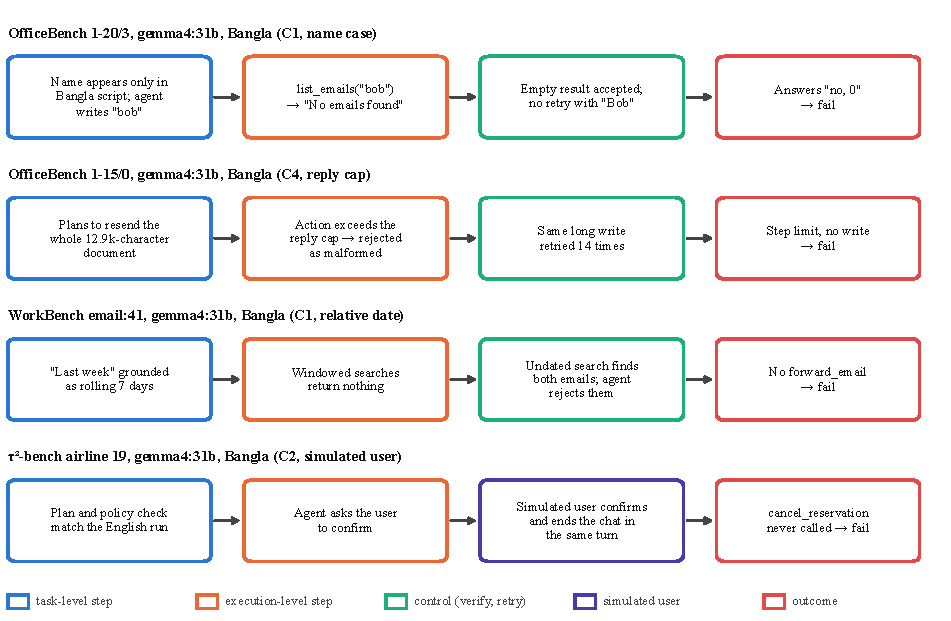
\includegraphics[width=\textwidth]{figures/fig_chains.pdf}
\caption{Four traced failure chains (Bangla runs whose English counterpart passes). Box colour
marks the kind of step; the confound class is given in parentheses.}
\label{fig:chains}
\end{figure*}

\section{Failure code book}
\label{app:codes}

\begin{table}[h]
\centering\small
\begin{tabular}{lp{5.1cm}}
\toprule
Code & Meaning \\
\midrule
BM  & Benchmark defect: a check or reference asks for something the task does not state \\
WC  & Wrong content: output exists, a value is wrong \\
SB  & Out of steps: hit the 20-step budget \\
PF  & Premature finish: declared done with a required output missing \\
TR  & Task read differently: a different operation from the one asked \\
FMT & Action format: could not produce a valid action \\
ER  & Empty result taken as ``nothing exists'' \\
\midrule
\multicolumn{2}{l}{\emph{Bangla-condition only}} \\
AL  & Answer language: correct answer in Bangla script, English check fails \\
NC  & Name case: a name rewritten from Bangla script with wrong case \\
WD  & Word choice when translating a literal back to English \\
TX  & Translation changed the task or a literal \\
\bottomrule
\end{tabular}
\caption{Failure codes. AL--TX cannot occur in the English condition and are the
language-specific modes discussed in Section~4.4.}
\label{tab:codebook}
\end{table}

\section{Task-type examples}
\label{app:taxexamples}

Table~\ref{tab:taxonomy} defines the nine task types of Section~\ref{sec:taxonomy} and their
typical failures; Table~\ref{tab:taxexamples} gives example tasks for each type.
\textsc{WorkBench} prompts are quoted from the task templates (message bodies shortened);
$\tau^2$-bench scenarios are paraphrased; for \textsc{TheAgentCompany} we give a summary of the
task and the checkpoints passed in each language.

\begin{table*}[t]
\centering\footnotesize
\begin{tabular}{L{2.8cm}L{5.5cm}L{6.3cm}}
\toprule
Task type & What the task asks & Typical failure (from trace review) \\
\midrule
Entity creation & Make one new record from details given in the request (send an
email, book a flight, open an account, write a document) & Wrong field values; on $\tau^2$
the wrong product or a skipped eligibility check; on TheAgentCompany an incomplete document \\
Single-target retrieval and action & Find the one record the request points to, then change
it (delete, update, return, move) & Wrong record or argument (an ID sent as a name), or stops
before the last step; on $\tau^2$ in Bangla often triggered by the simulated customer \\
Multi-target and batch operations & Select every record that matches conditions, or make
several changes in one request & Does part of the job, misses a matching item, or ends the
conversation early \\
Temporal reasoning & Work out free slots, relative dates or time shifts & Wrong slot,
``due today'' counted as overdue, or a Bangla date phrase misread \\
Data analysis and QA & Compute numbers from data, chart them, or look something up and
answer & Wrong metric or number, file not reachable (TheAgentCompany), result not checked \\
Conditional decision-making & Check a condition or policy first; act only if it holds,
otherwise refuse, do nothing or escalate & Acts before checking, gives in to a pushy
customer, or does not escalate \\
Cross-tool composition & Take a value from one tool and use it as input to another & Passes
the wrong value from the first tool to the second \\
Interpersonal coordination & Talk to coworkers in chat to obtain information or agreement &
Stops after the first reply and never follows up with a coworker who did not answer \\
System setup and troubleshooting & Install software, or walk a user through fixing a device
& Skips the final check, uses the wrong tool, or gives up when several faults are present \\
\bottomrule
\end{tabular}
\caption{The nine task types.}
\label{tab:taxonomy}
\end{table*}

\begin{table*}[t]
\centering\footnotesize
\begin{tabular}{L{2.8cm}L{12.0cm}}
\toprule
Task type & Examples \\
\midrule
Entity creation & \textit{WorkBench email:20}: ``I need to send an email to kofi saying `\ldots' and
title it `Task Update on Improve UX of onboarding process'. Can you do that?''
\textit{$\tau^2$ airline 8}: book a one-way flight from ORD to PHL on May 26 with an extra
passenger. \textit{TheAgentCompany hr-new-grad-job-description}: write a new-grad job
description from a template and a requirements file and save it on the cloud drive (EN 3/3,
BN 1/3). \\
Single-target & \textit{WorkBench email:6}: ``Delete my last email from chenwei.''
\textit{$\tau^2$ airline 16}: change an upcoming ATL--PHL trip to the cheapest Economy (not
Basic Economy) flight on the next day. \textit{TheAgentCompany admin-remove-pages-pdf}:
download a PDF from the cloud drive, remove pages and save the result (EN 1/3, BN 0/3). \\
Multi-target and batch & \textit{WorkBench email:41}: forward all emails from anaya sent last
week about `Update on Board of Directors Conclave' to nadia. \textit{WorkBench crm:77}: move
all customers who have not responded to a software proposal in 6 weeks to lost.
\textit{$\tau^2$ airline 22}: change the passenger, upgrade to economy and add 3 checked bags
in one request. \\
Temporal reasoning & \textit{WorkBench multi\_domain:84}: if olga has overdue tasks, book a
half-hour meeting `Catch up on overdue tasks' at the earliest time the user is free tomorrow.
\textit{TheAgentCompany admin-arrange-meeting-rooms}: find the minimum number of meeting rooms
for six teams' overlapping meetings (EN 0/2, BN 0/2). \\
Data analysis and QA & \textit{WorkBench analytics:20}: plot the distribution of engaged users
and total visits between November 5 and November 21. \textit{$\tau^2$ airline 3}: tell the
customer how many suitcases the reservation allows (the agent must verify that the customer is
Silver, not Gold). \textit{TheAgentCompany ds-answer-numerical-data-question}: answer numeric
questions about a spreadsheet (EN 0/6, BN 0/6). \\
Conditional decisions & \textit{WorkBench analytics:119}: make bar charts of social media and
search engine traffic over the last 4 weeks if social media brought more traffic.
\textit{$\tau^2$ airline 26}: refuse a cancellation with refund when the policy criteria are
not met. \textit{TheAgentCompany qa-escalate-emergency}: report a security bug and escalate
to the manager if the developer does not reply (EN 2/3, BN 2/3). \\
Cross-tool composition & \textit{WorkBench multi\_domain:25}: find the email from November 20
about `Task Update on Implement payment gateway API' and schedule a 30-minute meeting with its
sender on December 18 at 12:30. \\
Interpersonal coord. & \textit{TheAgentCompany admin-ask-for-meeting-feedback}: ask coworkers
for feedback on a meeting and record it in a spreadsheet (EN 6/6, BN 4/6). \\
System setup and troubl. & \textit{TheAgentCompany sde-install-go}: install the Go toolchain
and put it on PATH (EN 2/2, BN 0/2 in one of two task sets). \textit{$\tau^2$ telecom-11}: the
customer cannot send MMS; three hidden faults (bad network preference, data mode off, roaming
disabled while abroad). \\
\bottomrule
\end{tabular}
\caption{Example tasks per type. Checkpoint counts for TheAgentCompany are given as passed/total.}
\label{tab:taxexamples}
\end{table*}

\end{document}
